% !TeX encoding = UTF-8
% !TeX spellcheck = en_GB
\documentclass[a4paper]{article}

\usepackage[utf8]{inputenc}
\usepackage[T1]{fontenc}
\usepackage{lipsum}
\usepackage{enumitem,kantlipsum}
\usepackage{verbatim}
\usepackage{graphicx}

\graphicspath{ {images/} }

\title{Pollution Detection System\\User Manual}
\author{PLA25}

\begin{document}

\maketitle
\vspace*{\fill}

\paragraph{Group members}
\begin{tabbing}
	Joey Blankendaal 	\` 	500778751 	\\
	Thom de Jong 		\` 	500778147 	\\
	Brian Karmelk 		\` 	500768939 	\\
	Matthijs Snijders 	\` 	500780453 	\\
	Martijn Vegter 		\` 	500775388
\end{tabbing}

\thispagestyle{empty}
\newpage

\tableofcontents
\newpage

\section{Introduction}

\subsection{Who are we?}
We are a group of students who go by the name of PLA25. We are currently studying at the Amsterdam University of Applied Sciences. Our group consists of software engineering and technical computing students.

\subsection{Our product}
The Pollution Detection System (PDS) is a web-based application that provides information about the pollution on earth. Both light pollution and air pollution are being monitored using this system.
\newline
\newline
The system uses so called "sensorhubs". Sensorhubs are a combination of multiple sensors inside of a box. These sensorhubs can be placed in a specific area to measure the pollution. These measurements can be monitored using the PDS website. This can be done by using the website's main feature, the map.
\newline
\newline
The system uses sensors that can be placed in a specific area to measure the pollution. These measurements can be monitored using the PDS website. This can be done by using the website's main feature, the map.

\newpage
\section{The website}
\subsection{Login and Logout}
The login page is simple, use your username and password to login to the website. The website uses a role system, which means there are two roles a user of the website can be. You're either an admin or a user. 

\begin{enumerate}[]
	\item Use the upper input field for your username.
	\item Use the lower one for your password.
	\item Finally, click the "login" button.
\end{enumerate}
\noindent
After completing these steps you are being redirected to the homepage.
\newline
\newline
On the top of this website there is a navigation bar, which is used to visit the several available pages. These pages include: the home page the map page and the admin page. The latter is only shown if the current user is an admin.
\newline
\newline
If you want to log out, simply click the logout button at the very end of the navigation bar.
\newline
\newline
Both the login page and home page contain buttons to switch between the languages Dutch and English.

\subsection{The homepage}
Once the user has logged in to the website the user will be redirected to the home page of our website. On the home page the user will see a navigation bar at the top of the web page. On the navigation bar there will be several buttons. These buttons vary per user depending if the user is a admin or a user. 
\newline
\newline
On the home page itself the user will see a short welcome message as well. In the welcome message we introduce the user to our website and explain the features we have on our website. The home page also contains links to our blog, GitHub and more information for help.
\pagebreak

\subsection{The map page}
This page is used for viewing the gathered data. The data is displayed on the map. This map is the website's main feature. It can be used when you want to view the data from the sensorhubs.
\newline
This page features a map which can show you all kinds of data regarding pollution. On the left side there is a sidebar. This sidebar contains many options that can be used, for example: filters with which you can enable the heatmap, light pollution map and more.
\newline
\newline
There is also a search bar. With the search bar certain places like cities and towns can be found. Also, it can find a specific location by entering coordinates into the search bar. You can also look for companies with the search bar functionalities.
\newline
On the bottom left corner of the map page you will find something called the time line. The time line gives you the possibility to look at the past days. When you change the date or the time on the time line the map will change to the according data and planet pictures.  
\newline
Below the timeline there's a button called map information. By clicking on this button, you are able to see a legend of each pollution-related layer in the map; the temperature chart with the color spectrum, the light bulb images displaying the intensity levels and the numerical standards of the gas concentration.
\newline
\newline
The user is also possible to zoom in and out of the map so that they can get a more precise look at the map itself. 
\newline
If a user clicks on one of the sensor hubs, they are able to see a timeline of graphs displaying the different types of pollution and how they changed overtime in the area of the sensor hub. These graphs are connected with the timeline in the options menu.
\newline

\subsubsection{The heatmap}
If you want to see the temperature measured by the sensorhubs, this is the right option.
The heatmap shows a representation of the temperature, using colors scaling from bright pink (cold) to red (warm). The colors are displayed on the map as a layer over the standard map.\begin{figure}[h!]
  \caption{The heatmap.}
  \centering
  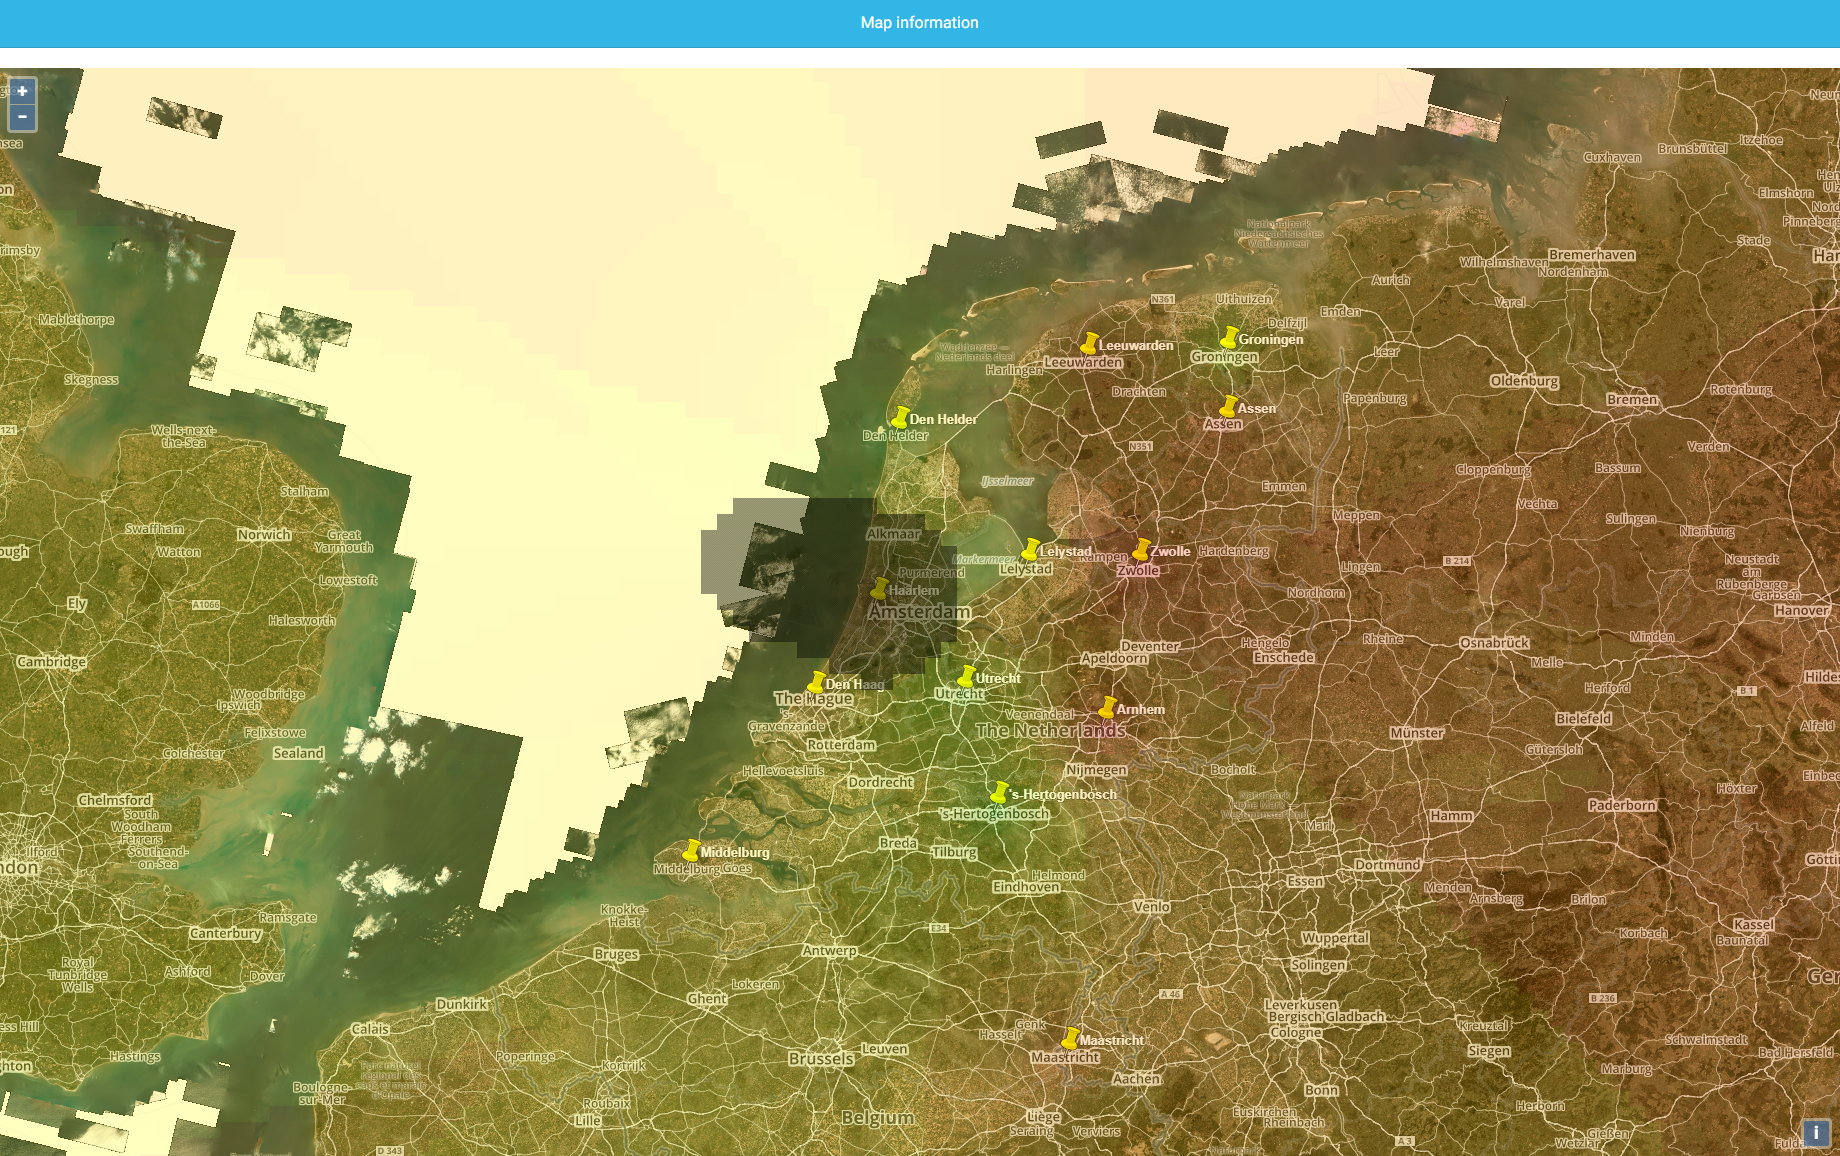
\includegraphics[width=1\textwidth]{heatmap}
\end{figure}
\newline
\subsubsection{The gas map} 
The gas map shows the amount of gass that is found on a specific location. The specific location will show the values given of the gss. On the map you will see a number which corresponds to an amount of pollution in the air due to gass.  

\subsubsection{The light map}
The light map shows the amount of light pollution at a specific location. The light pollution is shown by a lamp icon. The lamp icon has lines above the lamp itself. This is used as our scale. So if the lamp icon has 0 lines it means there isn't any pollution. But if there are 7 lines above the lamp icon it means that there is a lot of pollution going on in the area.

\newpage
\subsection{The admin page}
This page is used to make changes to the system, e.g. user management. Just like the name says, this page is only available for admins. On this page you can change a user's data or that of a sensorhub.
\newline
\newline
This page shows two tables. One table for the Users and one for the sensorhubs. With admin rights the user can change the data inside of these tables.
\newline
\newline
For example, the Users table contains data of all the users. With the add button you can add a user and with the delete button behind a specific user you can delete it. Then there is the edit button. The edit button is used to edit the profile of a specific user.
\newline
\newline
The sensorhub table simply shows the location of the used sensorhubs with pinpoints. The sensorhub table also contains the same buttons as the users table does.
\newline
\newline
At the top of the admin page admins are able to change the logo they have the website. There are two buttons, one is named "Bestand kiezen" and the other is called "Upload".  With the bestand kiezen button admins are able to choose a picture from their computer. And with the Upload admins are able to change the logo of the website with the picture they just selected through the Bestand kiezen button.
\newline
\newline
In the sensorhub table there is also a button called "details". When you press on the details button you will be redirected to a different page. On this page you will see all the values in a table of that specific location. On the side of the table you will see a chart. On the chart you will see the same data as in the table but instead of in a table in a chart.

\newpage
\section{Further help}
PLA25 is responsible for making this web application. If any bugs are to be found, please do contact us.
Also contact us if any further help is needed or something is not yet clear.

\end{document}
